%Esempio rapprsentare l'automa per disegnare w = 0^n 10 0^m 1^k
\documentclass{report}
\usepackage[T1]{fontenc}
\usepackage[utf8]{inputenc}
\usepackage{tikz}
\usetikzlibrary{automata,positioning}

\begin{document}
\begin{tikzpicture}[shorten >=1pt,node distance=3cm, on grid,auto]
  \node[state,initial] (q_0) {$q_0$};
  \node[state] (q_1) [right of= q_0]{$q_1$};
  \node[state,accepting] (q_2) [above right of = q_1] {$q_2$};
  \node[state] (q_E) [below right of = q_1] {$q_E$};

  \path[->]
  (q_0) edge  [loop above] node {0} ()
        edge  node [swap] {1} (q_1)
  (q_1) edge  node  {0} (q_2)
        edge  node {1} (q_E)

  (q_2) edge [loop above] node {0,1} ()
        
  (q_E) edge [loop above] node {0,1} ();      
        
\end{tikzpicture}

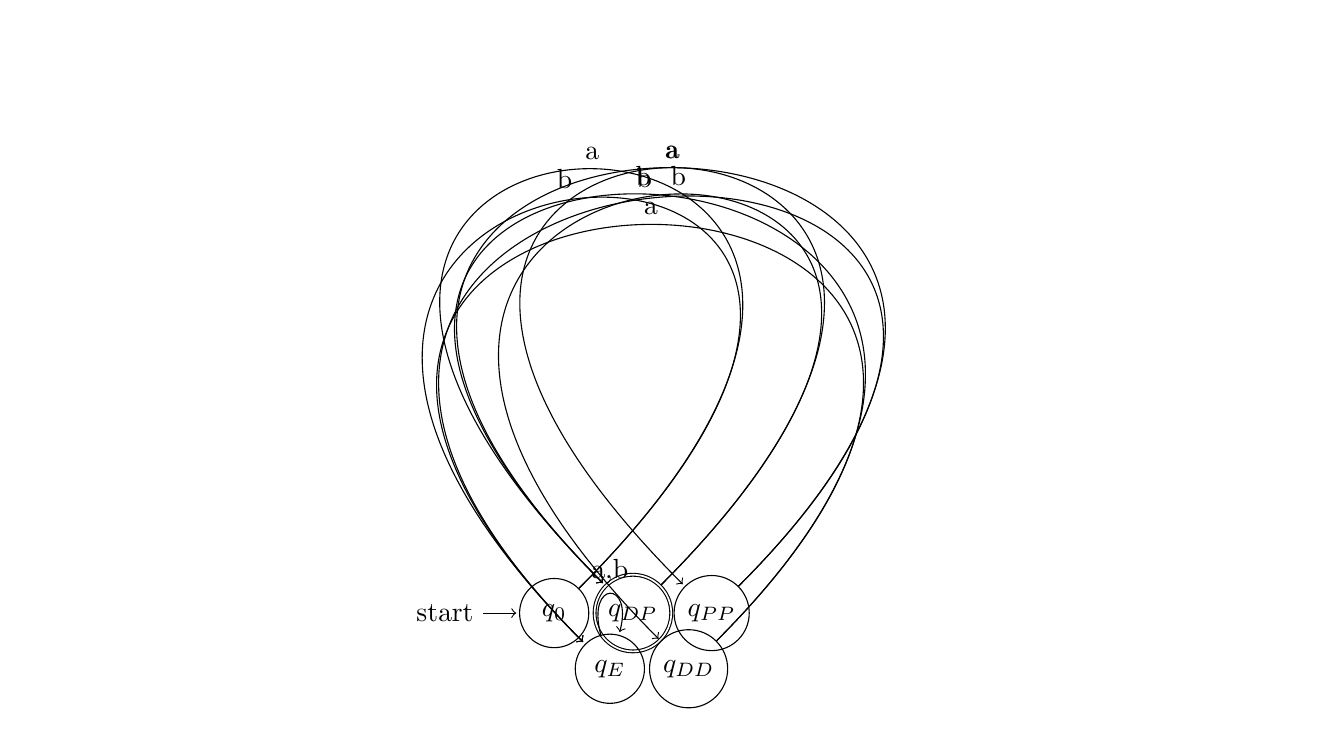
\begin{tikzpicture}[shorten >=1pt, distance = 10cm,on grid, auto]
  \node[state,initial] (q_0) {$q_0$};
  \node[state,accepting] (q_{DP}) [right of= q_0] {$q_{DP}$};
  \node[state] (q_E) [below right of= q_0] {$q_E$};
  \node[state] (q_{DD}) [below right of= q_{DP}] {$q_{DD}$};
  \node[state] (q_{PP}) [right of= q_{DP}] {$q_{PP}$};

  \path[->]
  (q_0) edge node [swap] {a} (q_{DP})
        edge node [swap] {b} (q_E)

  (q_{DP}) edge node [swap] {a} (q_{PP})
          edge node [swap] {b} (q_{DD})

  (q_{DD}) edge node [swap] {b} (q_{DP})
          edge node [swap] {a} (q_E)

  (q_{PP}) edge node [swap] {a} (q_{DP})
          edge node [swap] {b} (q_E)

  (q_E) edge [loop above] node {a,b} ();
\end{tikzpicture}

%Automa che termina per d con un numero pari di d

%Automa per disegnare aa^*cc^*d
\begin{tikzpicture}[shorten >= 1pt, distance = 10cm, on grid, auto]
  \node[state,initial] (q_0) {$q_0$};
  \node[state] (q_1) [right of = q_0] {$q_1$};
  \node[state] (q_E) [below right of= q_0] {$q_E$};
  \node[state] (q_2) [right of = q_1] {$q_2$};
  \node[state,accepting] (q_3) [right of = q_2] {$q_3$};

  \path[->]
  (q_0) edge node [swap] {a} (q_1)
        edge node [swap] {b,c,d} (q_E)

  (q_1) edge [loop above] node {a} ()
        edge node [swap] {c} (q_2)
        edge node [swap] {b,d} (q_E)

  (q_2) edge [loop above] node {c} ()
        edge node [swap] {d] (q_3)
        edge node [swap] {a,b} (q_E)
        (q_3) edge node [swap] {a,b,c,d} (q_E)
  (q_E) edge [loop above] node {a,b,c,d} ();
\end{tikzpicture}
\end{document}







































    1\4'
    
